
\section{Classified Performance Evaluation of Image-Based VTON}

\subsection{Image-based VTON algorithms}

In this Section, we started with evaluating the 2D image based VTON algorithms using a try-on cloth and a target human image. The human representation is composed of 1) heat maps for each joints 2) silhouette of human body, and 3) face and skin pixels patches (non-cloth and human identity area). It is assumed that the target human image is pre-processed for a cloth agnostic human representation by a human pose estimation like OpenPose\cite{Cao2018OpenPoseRM} and human parsing like LIP \cite{Liang2018LookIP}. % the algorithms 
We use the same dataset collected by Han et al. used in VITON\cite{Han2017VITONAI} and CP-VTON\cite{Wang2018TowardCI} papers. Here we include the SCM based-VTON, VITON \cite{Han2017VITONAI}, and  CP-VTON \cite{Wang2018TowardCI}. We included the SCM based algorithm  for a representative of non deep learning algorithm.

For clear notation, $C_i \in R^{H \times W \times3} $ denotes the try-on input cloth image 
and $ H_t = (J_t, R_t, S_t)$ is a human representation, 
where $ J_t \in R^{H \times W \times J}$, $R_t \in R^{H \times W \times 3}$, and $ S_t \in R^{H \times W}$ are a joint heat-map, residual (e.g hands, faces, hairs) color pixel images, and body shape silhouette merged human parsing segmentations from a human image $I_i$, respectively.    

The previous algorithms are mostly composed of two stages: (1) cloth warping step that warps the try-on cloth to align with the pose and shape of the target model (called GMM in CP-VTON \cite{Wang2018TowardCI}: geometric Manipulation Module), and (2) blending step that blends the warped cloth onto the target human image (called TON in CP-VTON: Try-On Network). 

The cloth warping step is done using SCM matching and transform from try-on cloth to the current, target cloth segmentation area, and the final VTON image is blended using simple alpha blending. For VITON and CP-VTON, a brief summary is as follows. For more details, the reader is refer to the original papers.


GMM of SCM-based VTON is defined by  
$
   \bold{\theta} = f_{SCM} (C_t, C_i)
$
and
$
   C_{warped} = f_{TPS}(\theta, Ci)
$.    
GMM of VITON is defined by 
$
   (I_{r}, M_{warped}) = f_{\theta, VITON} (H_t, C_i) 
$
and the loss function for training, 
\begin{equation}
   L_{GMM}^{VITON} =   \sum_{i=0}^{5} \lambda_i || \phi (I_r) - \phi (I_i)||  + 
   ||M_{C_{warped}} -  M_{C_t}||_1 .
\end{equation}

GMM of CP-VTON, GMM is defined by 
$  
   \bold{\theta} = f_{\theta} ( f_H (H_t), f_C(C_i) )
$
and
$
   C_{warped} = f_{TPS}(\theta, Ci).
$    
with the training loss function
\begin{equation}
   L_{GMM}^{CP-VTON} =  \sum ||C_{warped}, C_t||_1
\end{equation}

% GMM
The VITON use an encoder-decoder network to generate the warped cloth mask. Then the estimated TPS parameter from SCM matching between the generated mask and input try-on cloth mask is applied to the input try-on cloth. This is because in general the generated images from an encoder-decoder network does not preserved the original cloth as well as the warped image by geometric transform. Instead, CP-VTON uses a CNN based correlation network to estimated the TPS parameter directly and use the estimated parameters for warping.   


TOM  of SCM-based VTON  is defined by 
$
   M = f_{TPS}(\theta, M_{Ci}),
$    
and 
$
   I_o = M \odot C_{warped}, + (1-M) \odot I_i 
$.
TOM of VITON is defined by 
$
   \bold{\theta} = f_{SCM} (M_{C_t}, M_{C_i})
$,
$
   C_{warped} = f_{TPS}(\theta, Ci)
$,    
$
 M = f_{TOM} ( I_{r1}, C_{warped} ) 
$, 
and 
$
   I_o = M \odot C_{warped}, + (1-M) \odot I_{r},
$
with the training loss function, 
\begin{equation}
   L_{TOM}^{VITON} = \lambda_{VGG} \sum_{i=3}^{5} \lambda_i || \phi_i(I_o) - \phi_i(I_t)||_{1}  + 
             \lambda_{warp}  || M ||_{1}  + 
             \lambda_{TV} || \nabla M||_{1}      
\end{equation}

TOM of CP-VTON is defined by 
$
 (M, I_r) = f_{TOM} ( H_t, C_{warped} )  
$
and 
$
   I_o = M \odot C_{warped} + (1-M) \odot I_r
$
with the training loss function, 
\begin{equation}
   L_{TOM}^{CP-VTON} = \lambda_{L1}  || I_o - I_t ||_1  + 
             \lambda_{VGG} \sum_{i=1}^{5} || \phi_i(I_o) - \phi_i(I_t)||_1  + 
             \lambda_{mask} || 1 - M ||_1      
\end{equation}



% TOM
In TOM, the blending step, VITON generates an alpha blending mask image, which is used when alpha-blended with warped try-on cloth and human input image. The authors of CP-VTON observed that the blending is not successful when the warped  cloth area does not align well with the target area of human image, and first generates a coarse VTON results in addition to the composition mask, and then alpha-blends the warped cloth and the coarse VTON image with the alpha-composition mask.       


Differently from other GAN applications where the main purpose is to generate an unseen, plausible image, VTON application needs to retain the original texture and shape of the input try-on cloth. Due to its higher performance and logical architecture, CP-VTON \cite{Wang2018TowardCI} has become the benchmark benchmark algorithm for the image-based VTON algorithms recently published 
% \cite{     }.  But we can not include them in this paper because the implementations are not available. However, we believe the works share the strength and problems with three algorithms examined here. 


%The previous and following in 2019 share same input image and information conditions with CP-VTON and compare the results with it.
% Add some paper summary after CP-VTON .... and explain the differences from our works.

 
\subsection{Sample Classification}

% The criteria for classification   
First of all, the criteria for classifying the experimental samples were divided according to the complexity of the try-on clothes and the target human. The target human images are classified according to the complexity of the degree of occlusion (B, OP, OB, OF), posture (P), and shape (S) of the target cloth area of the human images. For the complexity of try-on cloths, we only uses the long sleeved (L) and short sleeved (S), because the length of sleeves is the biggest component in cloth warping and the used dataset does not have full diversity in cloth  style.    

%The degree of obscuration is a factor that affects the accuracy of the object of deformation, the posture is the degree of deformation, and the complexity of the clothes means the processing complexity of the clothes themselves.
%However, it is included in the range of classification, but not included in the actual experiment is shown in parentheses. Excluded conditions are those that are not included in the test data or that the evaluation is considered to be complex in the current technology. Based on this, six cases were classified as follows.

\begin{itemize}

\item[$\bullet$] BS : no or little occlusion and posture (Short sleeved clothes)
\item[$\bullet$] BL: no or little occlusion and posture (Long sleeved clothes)
\item[$\bullet$] OP: the target cloth area in a human image Occluded Partially by her/his hair and arms
\item[$\bullet$] OB: a large part of the clothing is Occluded by her/his Bottoms.
\item[$\bullet$] OFS: the target cloth area covered by the arms (with long sleeve and short sleeve)
\item[$\bullet$] OFS: the target cloth area Occluded in Front by her/his arms (Short sleeved clothes)
\item[$\bullet$] OFL: the target cloth area Occluded in Front by her/his arms (Long sleeved clothes)

\item[$\bullet$] P:  a large Posture deformation (e.g. a large movement of the arm or twisted or lateral posture)
\item[$\bullet$] S:  a large body shape change  (over-weighted or pregnant)

\end{itemize}

The cloth shape in the VITON dataset are mostly simple in shape and texture, e.g. a T-shirt (without a collar) of  monochromatic or monotone patterns. Even though it is clearly biased dataset, it is also not easy to define the un-biased one. Although all 2023 test images are used for experiment, some categories, e.g. S, does not have only small samples. But the trends of results in each category are very clear. 


 
 
\subsection{Result} 



For evaluation of performance, we used same cloth re-try on and new cloth try-on. 
The same cloth re-try-on experiment are done for quantitative evaluation of the algorithm with the ground truth results. In the same clothing experiment, we evaluate the cloth warping step performance using IoU (Intersection over Union) and the blending step performance using average SSIM (Structured SIMilarity index).

\begin{equation}
 IoU = \frac{ \hat{M}_{C_{warped}} \cap M_{C_{GT}}}
            { \hat{M}_{C_{warped}} \cup M_{C_{GT}}},
\end{equation} 
where $\hat{M}_{C_{warped}}$ and $M_{C_{GT}}$ are the estimated warped cloth's mask and the cloth area in the target human image, respectively. 

\begin{equation}
 SSIM = \frac{ ( 2 \mu_x \mu_y + c_1 )(2 \sigma_{xy} + c_2) }
             { ( \mu^2_x + \mu^2_y +c_1) ( \sigma^2_x + \sigma^2_y + c_2)}, 
\end{equation}
where we used default parameters for radius, $c_1$, $c_2$, and $c_3$. 

The experiment results are summarized as follows:

\begin{itemize}

\item[$\bullet$] BS $\&$ BL : All three algorithms show similar pattern. They generates natural synthesized VTON images for short-sleeved cloth, but show noticeable misalignment of warped cloth sleeves with the human image for long sleeved clothes. This larger misalignment in sleeve part can be explained by the fact that the matching and deformation are mainly done globally based on the whole silhouette, but not optimized for local deformation in the sleeves. 
TOM stages of VITON and CP-VTON can hide this misalignment to some degree by blending the un-covered target cloth area. However note that TOM networks can mimics but cannot retain the original cloth texture. 

\item[$\bullet$] OP: Partial occlusion by hair and other parts causes wrong human silhouette for GMM stage, which is designed for cloth-agnostic silhouette. All three algorithms affected this strongly. 

\item[$\bullet$] OB: The bottom occlusion cause SCM GMM generate unnatural deformation for long cloths. It is because SCM algorithm does not distinguish between deformation and occlusion and use the target cloth area directly for matching. In contrast to SCM-based GMM, VITON and CP-VITON GMMs use cloth-agnostic silhouettes and the effects are no or negligible.  

\item[$\bullet$] OF: GMM cannot generate natural warped clothes for long-sleeved clothes due to the limitations in matching and deformation.  TOM of all algorithms cannot generate the composition mask so the arm area gets blurred.  

\item[$\bullet$] P: All three algorithms fails to generate the warped clothes, but Interestingly the blending stage synthesizes the cloth color and texture to some degree. Nevertheless, the synthesize texture seldom align with original textures. As described  below, this is one of inherent and critical limitations of image based VTON approach.  


\item[$\bullet$] S: In VITON dataset, the matching cloth images for the human image of large or pregnant person are also large so the effects is not serious for the same cloth re-try-on.
\end{itemize}

 
 For new cloth try-on experiments, we provide visual analysis results. The wearing of a new cloth is, in effect, the ultimate result of the application. As above, an objective evaluation is not possible with VITON dataset. In the section 3, we compare the CP-VTON result and our proposed one with Inception Score (IS),too.
 
\begin{itemize}

\item[$\bullet$] BS $\&$ BL: The clothing deformation itself shows good results similar to the result with same cloths, but there are some differences according to the algorithms in the synthesis. When switching from long to short sleeves, SCM does not restore the skin area, whereas VITON and CP-VTON can generate the skin area for the revealing bare arm. Especially due to the coarse VTON output of it, CP-VTON can generate much clear skin area.

\item[$\bullet$] OP: The performance was similar to that of the same clothes.

\item[$\bullet$] OBS $\&$ OBL: The same characteristics as the same image, that is, the SCM shows a problem that can not distinguish the occlusion and deformation.

\item[$\bullet$] OF: As in the case of the same cloth, in the case of SCM, the synthesis algorithm needs to be improved when switching from the short sleeved to the long sleeved.

\item[$\bullet$] P: As in the case of the same cloth, there was a large error in deformation and alignment of the try-on cloth.

\item[$\bullet$] S: Results shows GMM, especially of VITON and CP-VTON, can warp the new cloth to the target human body shape change, 

\end{itemize}

%In addition to the analysis of each condition in addition to the analysis of each condition, it can be seen that there are the following big features. First, it was confirmed that the shape change of clothes by GMM has an influence on the current wear clothes. The reason is that SCMM uses the area of the current costume, and deep learning methods use the body itself, but the area of the current costume is reflected in the correct answer mask used in the learning process.


\begin{figure}
\centering
%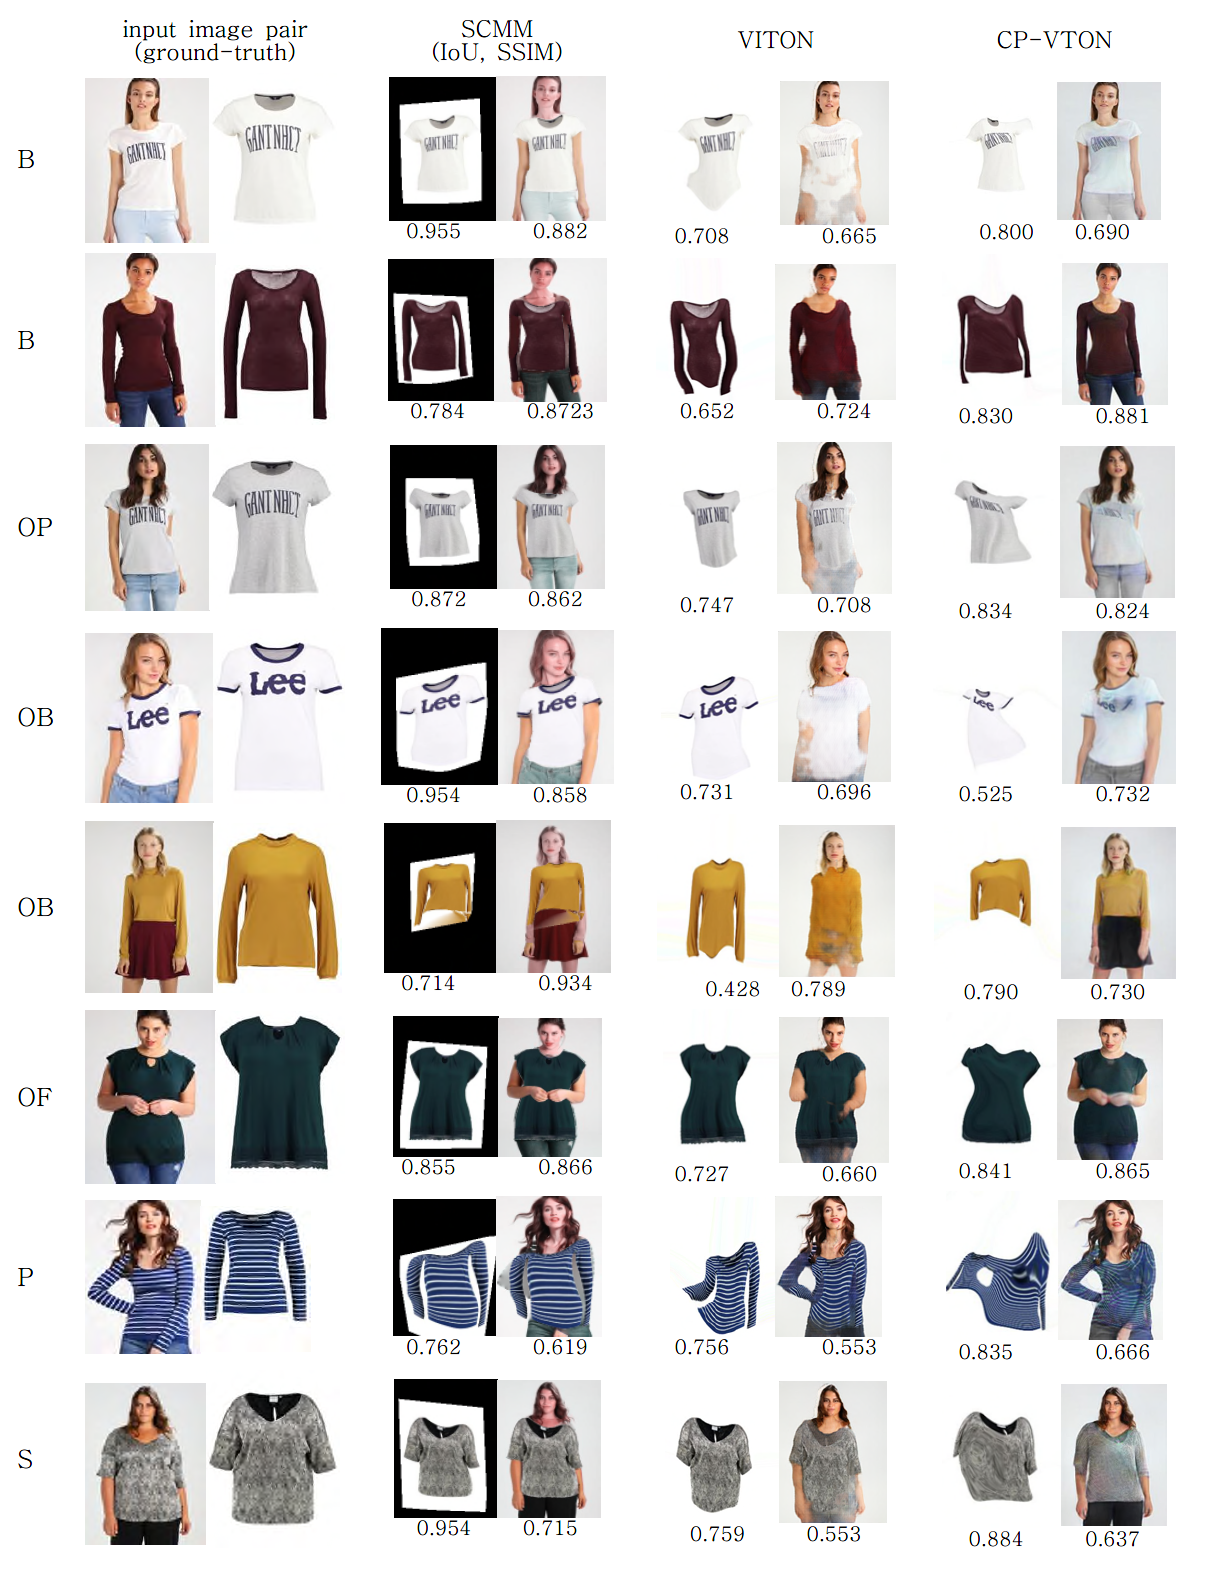
\includegraphics[height=13.5cm, scale=1]{figures/2dvton_same.png}   
\begin{tabular}{cccccccccccc}
 & \multicolumn{2}{c}{input}   &  \multicolumn{2}{c}{SCM-based}    & \multicolumn{2}{c}{VITON}    &  \multicolumn{2}{c}{CP-VTON}  & \multicolumn{2}{c}{CP-VTON+ (ours)} \\
BS &
   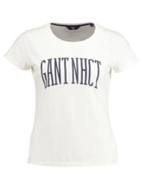
\includegraphics[ width=1cm, keepaspectratio]{figures/same/bsc.png} &
   
\includegraphics[ width=1cm, keepaspectratio]{figures/same/bsh.png} &
   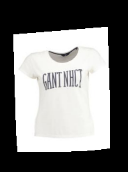
\includegraphics[ width=1cm, keepaspectratio]{figures/same/bsscmc.png} &
   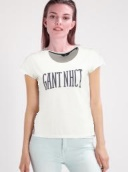
\includegraphics[ width=1cm, keepaspectratio]{figures/same/bsscmh.png} &
   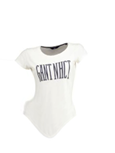
\includegraphics[ width=1cm, keepaspectratio]{figures/same/bsvitonc.png} &
   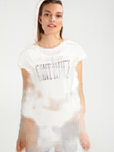
\includegraphics[ width=1cm, keepaspectratio]{figures/same/bsvitonh.png} &
   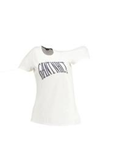
\includegraphics[ width=1cm, keepaspectratio]{figures/same/bsvtonc.png} &
   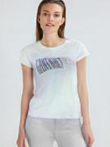
\includegraphics[ width=1cm, keepaspectratio]{figures/same/bsvtonh.png} &
   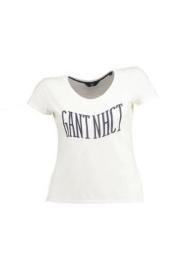
\includegraphics[ width=1cm, keepaspectratio]{figures/same/bsvton+c.png} &
   
\includegraphics[ width=1cm, keepaspectratio]{figures/same/bsvton+h.png}  \\
 &&& 
   0.955 & 0.882 &
   0.708 & 0.665 & 
   0.800 & 0.690 &
   0.933 & 0.785\\   
   
BL &
   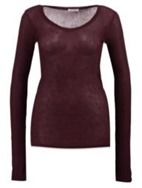
\includegraphics[ width=1cm, keepaspectratio]{figures/same/blc.png} &
   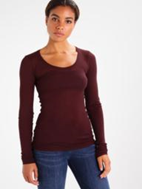
\includegraphics[ width=1cm, keepaspectratio]{figures/same/blh.png} &
   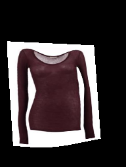
\includegraphics[ width=1cm, keepaspectratio]{figures/same/blscmc.png} &
   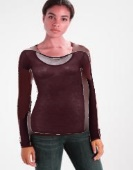
\includegraphics[ width=1cm, keepaspectratio]{figures/same/blscmh.png} &
   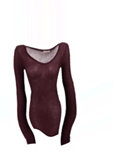
\includegraphics[ width=1cm, keepaspectratio]{figures/same/blvitonc.png} &
   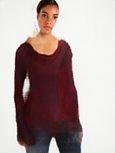
\includegraphics[ width=1cm, keepaspectratio]{figures/same/blvitonh.png} &
   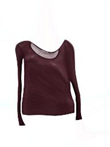
\includegraphics[ width=1cm, keepaspectratio]{figures/same/blvtonc.png} &
   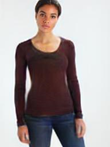
\includegraphics[ width=1cm, keepaspectratio]{figures/same/blvtonh.png} &
   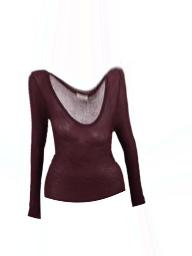
\includegraphics[ width=1cm, keepaspectratio]{figures/same/blvton+c.png} &
   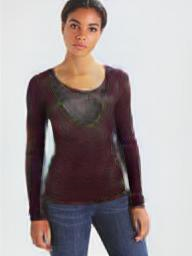
\includegraphics[ width=1cm, keepaspectratio]{figures/same/blvton+h.png}  \\
 &&& 
     0.784 & 0.872 &
     0.652 & 0.724 &
     0.830 & 0.881 &
     0.862 & 0.878\\

OP &
   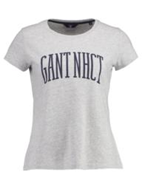
\includegraphics[ width=1cm, keepaspectratio]{figures/same/opc.png} &
   
\includegraphics[ width=1cm, keepaspectratio]{figures/same/oph.png} &
   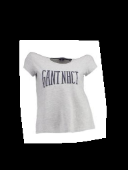
\includegraphics[ width=1cm, keepaspectratio]{figures/same/opscmc.png} &
   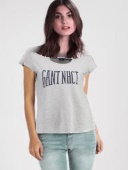
\includegraphics[ width=1cm, keepaspectratio]{figures/same/opscmh.png} &
   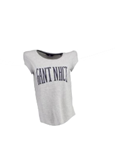
\includegraphics[ width=1cm, keepaspectratio]{figures/same/opvitonc.png} &
   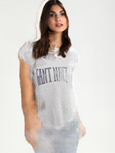
\includegraphics[ width=1cm, keepaspectratio]{figures/same/opvitonh.png} &
   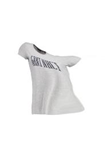
\includegraphics[ width=1cm, keepaspectratio]{figures/same/opvtonc.png} &
   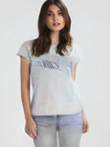
\includegraphics[ width=1cm, keepaspectratio]{figures/same/opvtonh.png} &
   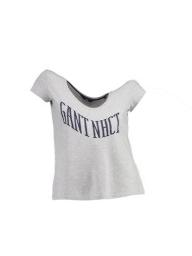
\includegraphics[ width=1cm, keepaspectratio]{figures/same/opvton+c.png} &
   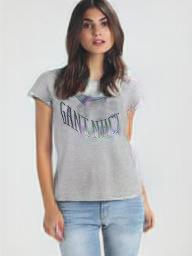
\includegraphics[ width=1cm, keepaspectratio]{figures/same/opvton+h.png}  \\
 &&&  
     0.872 &  0.862	&
     0.747 &  0.708	&
     0.834 &  0.824 &	  
     0.877 &  0.863\\
     
     

OBS &
   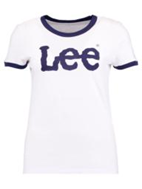
\includegraphics[ width=1cm, keepaspectratio]{figures/same/obsc.png} &
   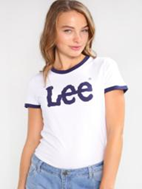
\includegraphics[ width=1cm, keepaspectratio]{figures/same/obsh.png} &
   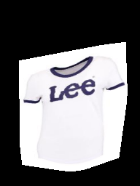
\includegraphics[ width=1cm, keepaspectratio]{figures/same/obsscmc.png} &
   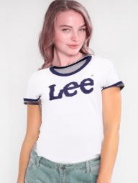
\includegraphics[ width=1cm, keepaspectratio]{figures/same/obsscmh.png} &
   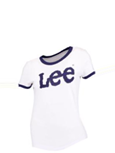
\includegraphics[ width=1cm, keepaspectratio]{figures/same/obsvitonc.png} &
   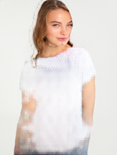
\includegraphics[ width=1cm, keepaspectratio]{figures/same/obsvitonh.png} &
   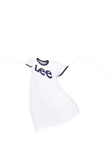
\includegraphics[ width=1cm, keepaspectratio]{figures/same/obsvtonc.png} &
   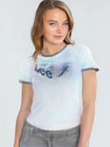
\includegraphics[ width=1cm, keepaspectratio]{figures/same/obsvtonh.png} &
   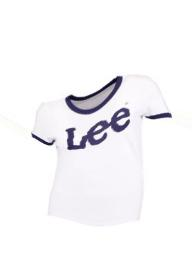
\includegraphics[ width=1cm, keepaspectratio]{figures/same/obsvton+c.png} &
   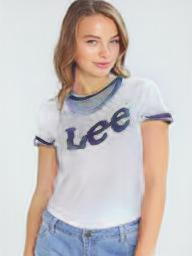
\includegraphics[ width=1cm, keepaspectratio]{figures/same/obsvton+h.png}  \\
 &&&  
      0.954  &       0.858	&  
       0.731 &        0.696	 & 
       0.525 &         0.732 &	  
           0.933 &       0.804\\
OBL &
   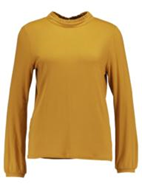
\includegraphics[ width=1cm, keepaspectratio]{figures/same/oblc.png} &
   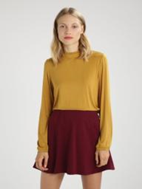
\includegraphics[ width=1cm, keepaspectratio]{figures/same/oblh.png} &
   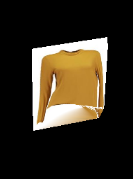
\includegraphics[ width=1cm, keepaspectratio]{figures/same/oblscmc.png} &
   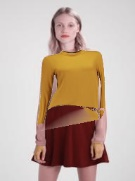
\includegraphics[ width=1cm, keepaspectratio]{figures/same/oblscmh.png} &
   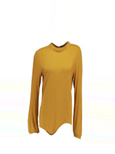
\includegraphics[ width=1cm, keepaspectratio]{figures/same/oblvitonc.png} &
   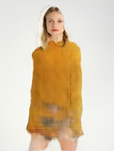
\includegraphics[ width=1cm, keepaspectratio]{figures/same/oblvitonh.png} &
   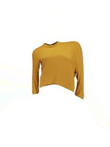
\includegraphics[ width=1cm, keepaspectratio]{figures/same/oblvtonc.png} &
   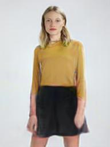
\includegraphics[ width=1cm, keepaspectratio]{figures/same/oblvtonh.png} &
   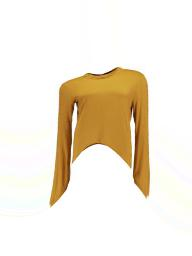
\includegraphics[ width=1cm, keepaspectratio]{figures/same/oblvton+c.png} &
   \includegraphics[ width=1cm, keepaspectratio]{figures/same/oblvton+h.png}  \\
&&&  
      0.714 &  0.934 &	  
      0.428 &  0.789 &	  
      0.790 &  0.730 &	  
      0.816 &  0.897\\

OF &
   \includegraphics[ width=1cm, keepaspectratio]{figures/same/ofc.png} &
   \includegraphics[ width=1cm, keepaspectratio]{figures/same/ofh.png} &
   \includegraphics[ width=1cm, keepaspectratio]{figures/same/ofscmc.png} &
   \includegraphics[ width=1cm, keepaspectratio]{figures/same/ofscmh.png} &
   \includegraphics[ width=1cm, keepaspectratio]{figures/same/ofvitonc.png} &
   \includegraphics[ width=1cm, keepaspectratio]{figures/same/ofvitonh.png} &
   \includegraphics[ width=1cm, keepaspectratio]{figures/same/ofvtonc.png} &
   \includegraphics[ width=1cm, keepaspectratio]{figures/same/ofvtonh.png} &
   \includegraphics[ width=1cm, keepaspectratio]{figures/same/ofvton+c.png} &
   \includegraphics[ width=1cm, keepaspectratio]{figures/same/ofvton+h.png}  \\
&&&  
     0.855 & 0.866 &	  
     0.727 & 0.660 &	  
     0.841 & 0.865 &	  
     0.847 & 0.874\\
P &
   \includegraphics[ width=1cm, keepaspectratio]{figures/same/pc.png} &
   \includegraphics[ width=1cm, keepaspectratio]{figures/same/ph.png} &
   \includegraphics[ width=1cm, keepaspectratio]{figures/same/pscmc.png} &
   \includegraphics[ width=1cm, keepaspectratio]{figures/same/pscmh.png} &
   \includegraphics[ width=1cm, keepaspectratio]{figures/same/pvitonc.png} &
   \includegraphics[ width=1cm, keepaspectratio]{figures/same/pvitonh.png} &
   \includegraphics[ width=1cm, keepaspectratio]{figures/same/pvtonc.png} &
   \includegraphics[ width=1cm, keepaspectratio]{figures/same/pvtonh.png} &
   \includegraphics[ width=1cm, keepaspectratio]{figures/same/pvton+c.png} &
   \includegraphics[ width=1cm, keepaspectratio]{figures/same/pvton+h.png}  \\
&&&  
     0.762 & 0.619 &	  
     0.756 & 0.553 &	  
     0.835 & 0.666 &	  
     0.841 & 0.663\\
S &
   \includegraphics[ width=1cm, keepaspectratio]{figures/same/sc.png} &
   \includegraphics[ width=1cm, keepaspectratio]{figures/same/sh.png} &
   \includegraphics[ width=1cm, keepaspectratio]{figures/same/sscmc.png} &
   \includegraphics[ width=1cm, keepaspectratio]{figures/same/sscmh.png} &
   \includegraphics[ width=1cm, keepaspectratio]{figures/same/svitonc.png} &
   \includegraphics[ width=1cm, keepaspectratio]{figures/same/svitonh.png} &
   \includegraphics[ width=1cm, keepaspectratio]{figures/same/svtonc.png} &
   \includegraphics[ width=1cm, keepaspectratio]{figures/same/svtonh.png} &
   \includegraphics[ width=1cm, keepaspectratio]{figures/same/svton+c.png} &
   \includegraphics[ width=1cm, keepaspectratio]{figures/same/svton+h.png}  \\
&&&  
      0.954 & 0.715	&  
      0.759 & 0.553	&  
      0.884 & 0.637 &	  
      0.888 & 0.652\\
\end{tabular}

\caption{Classified Evaluation of Image-based VTONs (same cloth re-try-on): left to right, input pairs, SCM-based results, VITON results, CP-VTON results, CP-VTON+ (ours) results.  The numbers below cloth and human images are IoU and SSIM, respectively. }
\label{fig:2dvton_same}
\end{figure}



\begin{figure}
\centering
%\includegraphics[height=13.5cm, scale=1]{figures/2dvton_diff.png}  %% TODO  

\begin{tabular}{cccccccccccc}

  &  \multicolumn{2}{c}{input}  & \multicolumn{2}{c}{SCM-based}   & \multicolumn{2}{c}{VITON}    &  \multicolumn{2}{c}{CP-VTON}  & \multicolumn{2}{c}{CP-VTON+ (ours)} \\
BS &
   \includegraphics[ width=1cm, keepaspectratio]{figures/new/bsc.png} &
   \includegraphics[ width=1cm, keepaspectratio]{figures/new/bsh.png} &
   \includegraphics[ width=1cm, keepaspectratio]{figures/new/bsscmc.png} &
   \includegraphics[ width=1cm, keepaspectratio]{figures/new/bsscmh.png} &
   \includegraphics[ width=1cm, keepaspectratio]{figures/new/bsvitonc.png} &
   \includegraphics[ width=1cm, keepaspectratio]{figures/new/bsvitonh.png} &
   \includegraphics[ width=1cm, keepaspectratio]{figures/new/bsvtonc.png} &
   \includegraphics[ width=1cm, keepaspectratio]{figures/new/bsvtonh.png} &
   \includegraphics[ width=1cm, keepaspectratio]{figures/new/bsvton+c.png} &
   \includegraphics[ width=1cm, keepaspectratio]{figures/new/bsvton+h.png}  \\
   
BL &
   \includegraphics[ width=1cm, keepaspectratio]{figures/new/blc.png} &
   \includegraphics[ width=1cm, keepaspectratio]{figures/new/blh.png} &
   \includegraphics[ width=1cm, keepaspectratio]{figures/new/blscmc.png} &
   \includegraphics[ width=1cm, keepaspectratio]{figures/new/blscmh.png} &
   \includegraphics[ width=1cm, keepaspectratio]{figures/new/blvitonc.png} &
   \includegraphics[ width=1cm, keepaspectratio]{figures/new/blvitonh.png} &
   \includegraphics[ width=1cm, keepaspectratio]{figures/new/blvtonc.png} &
   \includegraphics[ width=1cm, keepaspectratio]{figures/new/blvtonh.png} &
   \includegraphics[ width=1cm, keepaspectratio]{figures/new/blvton+c.png} &
   \includegraphics[ width=1cm, keepaspectratio]{figures/new/blvton+h.png}  \\

OP &
   \includegraphics[ width=1cm, keepaspectratio]{figures/new/opc.png} &
   \includegraphics[ width=1cm, keepaspectratio]{figures/new/oph.png} &
   \includegraphics[ width=1cm, keepaspectratio]{figures/new/opscmc.png} &
   \includegraphics[ width=1cm, keepaspectratio]{figures/new/opscmh.png} &
   \includegraphics[ width=1cm, keepaspectratio]{figures/new/opvitonc.png} &
   \includegraphics[ width=1cm, keepaspectratio]{figures/new/opvitonh.png} &
   \includegraphics[ width=1cm, keepaspectratio]{figures/new/opvtonc.png} &
   \includegraphics[ width=1cm, keepaspectratio]{figures/new/opvtonh.png} &
   \includegraphics[ width=1cm, keepaspectratio]{figures/new/opvton+c.png} &
   \includegraphics[ width=1cm, keepaspectratio]{figures/new/opvton+h.png}  \\

OBS &
   \includegraphics[ width=1cm, keepaspectratio]{figures/new/obsc.png} &
   \includegraphics[ width=1cm, keepaspectratio]{figures/new/obsh.png} &
   \includegraphics[ width=1cm, keepaspectratio]{figures/new/obsscmc.png} &
   \includegraphics[ width=1cm, keepaspectratio]{figures/new/obsscmh.png} &
   \includegraphics[ width=1cm, keepaspectratio]{figures/new/obsvitonc.png} &
   \includegraphics[ width=1cm, keepaspectratio]{figures/new/obsvitonh.png} &
   \includegraphics[ width=1cm, keepaspectratio]{figures/new/obsvtonc.png} &
   \includegraphics[ width=1cm, keepaspectratio]{figures/new/obsvtonh.png} &
   \includegraphics[ width=1cm, keepaspectratio]{figures/new/obsvton+c.png} &
   \includegraphics[ width=1cm, keepaspectratio]{figures/new/obsvton+h.png}  \\

OBL &
   \includegraphics[ width=1cm, keepaspectratio]{figures/new/oblc.png} &
   \includegraphics[ width=1cm, keepaspectratio]{figures/new/oblh.png} &
   \includegraphics[ width=1cm, keepaspectratio]{figures/new/oblscmc.png} &
   \includegraphics[ width=1cm, keepaspectratio]{figures/new/oblscmh.png} &
   \includegraphics[ width=1cm, keepaspectratio]{figures/new/oblvitonc.png} &
   \includegraphics[ width=1cm, keepaspectratio]{figures/new/oblvitonh.png} &
   \includegraphics[ width=1cm, keepaspectratio]{figures/new/oblvtonc.png} &
   \includegraphics[ width=1cm, keepaspectratio]{figures/new/oblvtonh.png} &
   \includegraphics[ width=1cm, keepaspectratio]{figures/new/oblvton+c.png} &
   \includegraphics[ width=1cm, keepaspectratio]{figures/new/oblvton+h.png}  \\

OF &
   \includegraphics[ width=1cm, keepaspectratio]{figures/new/ofc.png} &
   \includegraphics[ width=1cm, keepaspectratio]{figures/new/ofh.png} &
   \includegraphics[ width=1cm, keepaspectratio]{figures/new/ofscmc.png} &
   \includegraphics[ width=1cm, keepaspectratio]{figures/new/ofscmh.png} &
   \includegraphics[ width=1cm, keepaspectratio]{figures/new/ofvitonc.png} &
   \includegraphics[ width=1cm, keepaspectratio]{figures/new/ofvitonh.png} &
   \includegraphics[ width=1cm, keepaspectratio]{figures/new/ofvtonc.png} &
   \includegraphics[ width=1cm, keepaspectratio]{figures/new/ofvtonh.png} &
   \includegraphics[ width=1cm, keepaspectratio]{figures/new/ofvton+c.png} &
   \includegraphics[ width=1cm, keepaspectratio]{figures/new/ofvton+h.png}  \\

P &
   \includegraphics[ width=1cm, keepaspectratio]{figures/new/pc.png} &
   \includegraphics[ width=1cm, keepaspectratio]{figures/new/ph.png} &
   \includegraphics[ width=1cm, keepaspectratio]{figures/new/pscmc.png} &
   \includegraphics[ width=1cm, keepaspectratio]{figures/new/pscmh.png} &
   \includegraphics[ width=1cm, keepaspectratio]{figures/new/pvitonc.png} &
   \includegraphics[ width=1cm, keepaspectratio]{figures/new/pvitonh.png} &
   \includegraphics[ width=1cm, keepaspectratio]{figures/new/pvtonc.png} &
   \includegraphics[ width=1cm, keepaspectratio]{figures/new/pvtonh.png} &
   \includegraphics[ width=1cm, keepaspectratio]{figures/new/pvton+c.png} &
   \includegraphics[ width=1cm, keepaspectratio]{figures/new/pvton+h.png}  \\

S &
   \includegraphics[ width=1cm, keepaspectratio]{figures/new/sc.png} &
   \includegraphics[ width=1cm, keepaspectratio]{figures/new/sh.png} &
   \includegraphics[ width=1cm, keepaspectratio]{figures/new/sscmc.png} &
   \includegraphics[ width=1cm, keepaspectratio]{figures/new/sscmh.png} &
   \includegraphics[ width=1cm, keepaspectratio]{figures/new/svitonc.png} &
   \includegraphics[ width=1cm, keepaspectratio]{figures/new/svitonh.png} &
   \includegraphics[ width=1cm, keepaspectratio]{figures/new/svtonc.png} &
   \includegraphics[ width=1cm, keepaspectratio]{figures/new/svtonh.png} &
   \includegraphics[ width=1cm, keepaspectratio]{figures/new/svton+c.png} &
   \includegraphics[ width=1cm, keepaspectratio]{figures/new/svton+h.png}  \\

\end{tabular}

\caption{Classified Evaluation of Image-based VTONs (new cloth try-on): left to right, input pairs, SCM-based results, VITON results, CP-VTON results, CP-VTON+ (ours) results.}
\label{fig:2dvton_diff}
\end{figure}

 
\subsection{Discussion}

% comparison between algorithm
Among the three algorithms used, CP-VTON shows the best performance in both same cloth re-try-on and new cloth try-on. However there are some notable observations. 

As for the warping step, interestingly, SCM-based GMM generates the best results in the alignment and deformation of the try-on clothes to the target human for the same cloth. This somewhat conflicting against \cite{Wang2018TowardCI} can be explained as follows. In \cite{Wang2018TowardCI}, they only considered new cloth try-on cases.  Note that SCM can use the ground truth target in same cloth re-try-on so that it can find better matching points. However, for the new cloth cases, when the shapes of new cloth and current clothes has big difference, the results get worse than the other methods.
  
And in general, CP-VTON GMM using CNN Geometry matching algorithm shows better results than VITON GMM. Since both CP-VTON and VITON use TPS algorithm, the difference comes from TPS parameter estimation step. We can conclude the CNN-based matching works better that of VITON. Nevertheless the matching is not very reliable and the warped cloth show strong distortion in texture, e.g. pattern and logos. 

Examination the sample they argued and tried to use cloth-agnostic human representation, the current VITON dataset target try-on area is dependent upon current cloth shape. Especially, the neck area pixels are labeled as background and some body areas are occluded by hairs or accessories (Figure \ref{fig:cpvtonissues}), which affects in cloth warping and blending. 

 
GMM module using Spatial Transform Network\cite{JaderbergSZK15} with TPS (Thin Plate Spline)\cite{Bookstein1989PrincipalWT} deformation cannot handle strong 3D deformation due to the target pose and also generates artifacts because of the person representation inputs. For example, hands-up and folded arms.  Note that many errors in the warping stage are often hidden in the blending stage when the target clothes are single-colored, which can be expected in practical conditions 
%(Fig. 3 (d)).

      
As for the blending stage, CP-VTON performs best among three algorithms. SCM generates clear texture but a noticeable cloth boundaries due to the binary mask used for blending.  CP-VTON generated much clearer cloth texture thanks to its composition mask and synthesized VTON result.

% 2.
%Secondly, 
All the other parts but the target cloth area, e.g. faces, hair, and arms, bottom-clothes have to be retained in blending stage. But other parts except face and hair are missing in CP-VTON\cite{Wang2018TowardCI} human representation and generated at blending stage, which is all right for general synthesis application but not desirable in VTON application (Figure \ref{fig:cpvtonissues}). 


% 3.
The texture is often not vivid, which is due to the unclear composition mask. Examining the original loss function of TOM network, the term for the composition alpha mask are poorly formulated as simple regularization loss $|| 1 - M_{o} ||_1$.   

%
%\begin{equation}
%L = \lambda_{L1} || I_0-I_{GT} ||_1 +  \lambda_{VGG} L_{VGG}+ \lambda_3 || 1 - M_{o} ||_1        
%\end{equation} 


%4. 
Fourthly, since no label in the area of warped cloth is the same color as background, white colored clothes are confused and improperly processed in the blending stage (Fig. 3 (c))


%All the used image-based algorithms shows similar trends in each input
%Even though the success and failure cases are presented and compared with other algorithms' results, the failure case analysis is not enough for understanding the origin of failure cases and therefore difficult to find the solution for them. A classified evaluation would be better for this understanding. Here we summarized the classified results from our another study. We classify input try-on cloth and target human images according to the posture and body type of the person, the degree of occlusion of the clothes, and the characteristics of the clothes. Quality is compared in IoU for the warping step and in SSIM for the final blending step for same cloth re-try-on cases. We also tested for the new cloth try-on cases but did not include here for limitation of spaces, and the same cloth cases are enough to explain the tendencies of the performances. Though in general CP-VTON generates the best quality image, the relative comparison is not the main purpose of the analysis. Please refer to Figure \ref{fig:classified2DVTONresult} for detailed results.

\begin{figure}
\centering
\includegraphics[height=6.5cm, scale=1]{figures/cpvtonissues.png}   % TODO
\caption{The issues in CP-VTON}
\label{fig:cpvtonissues}
\end{figure}



%Especially note that the warped cloth are often too much different for desired shape. It is originated two facts. First the 3D deformation that any 2D deformation including non-rigid transform such as TPS is quite limited, especially any 2D deformation cannot handle when the two area in the original image are overlapped in the destination images. There for when the arms of long sleeved cloth occlude the main body, 2D warping cannot approximate the 3D deformation properly. Second, the deformation needs corresponding points  between the source nd target image. The cloth are extremely difficult object to find the corresponding points. The STN (spatial transform network)\cite{JaderbergSZK15} and SCM (shape context matching)\cite{BelongieMP02} cannot find the corresponding points when the target cloth and original cloth has different shapes. In conclusion, the 2D image based algorithm has serious limitation in the range of applications. It can apply to the mild posed target human only and simple short sleeved cloth, mainly because the inherent limitation of 2D deformation method including non-rigid ones, and the poor performance of matching algorithm.  To overcome this limitation, we consider to model the try-on cloth into 3D model and apply the 3D deformation
